\documentclass[12pt, a4paper]{article}
\usepackage{amsmath, amssymb, amscd, amsthm, amsfonts}
\usepackage{graphicx}
\usepackage{hyperref}
\usepackage{url}
\usepackage[utf8]{inputenc}
\usepackage{biblatex}
\usepackage[top=2.5cm, bottom=2.5cm, left=2.5cm, right=2.5cm]{geometry}
\usepackage{minted}
\usepackage{amsmath}
\usepackage{hyperref}
\usepackage[selection]{placeins}
\usepackage{indentfirst}
\usepackage[document]{ragged2e}
\usepackage{float}
\usepackage{pdfpages}
\newcommand{\tsp}{\textsuperscript}
\newcommand{\tsb}{\textsubscript}
\newtheorem{theorem}{Theorem}
\newtheorem{lemma}[theorem]{Lemma}
\newtheorem{conjecture}[theorem]{Conjecture}
\newcommand{\rr}{\mathbb{R}}
\newcommand{\al}{\alpha}
\DeclareMathOperator{\conv}{conv}
\DeclareMathOperator{\aff}{aff}
\addbibresource{references.bib}

\begin{document}

\justifying 
\title{Equivalent Circuits}
\author{Miriam Bonello}
\date{10th November 2022}

\maketitle 

\begin{abstract}
\end{abstract}

\section*{Introduction}\label{section-introduction}
\subsection*{Henlo} 

he wins in spa he wins in monza charles leclerc win the italian grand prix 
\medskip 

hello from the other side 

\subsection*{Figures}\begin{figure}[h!]
    \begin{center}
    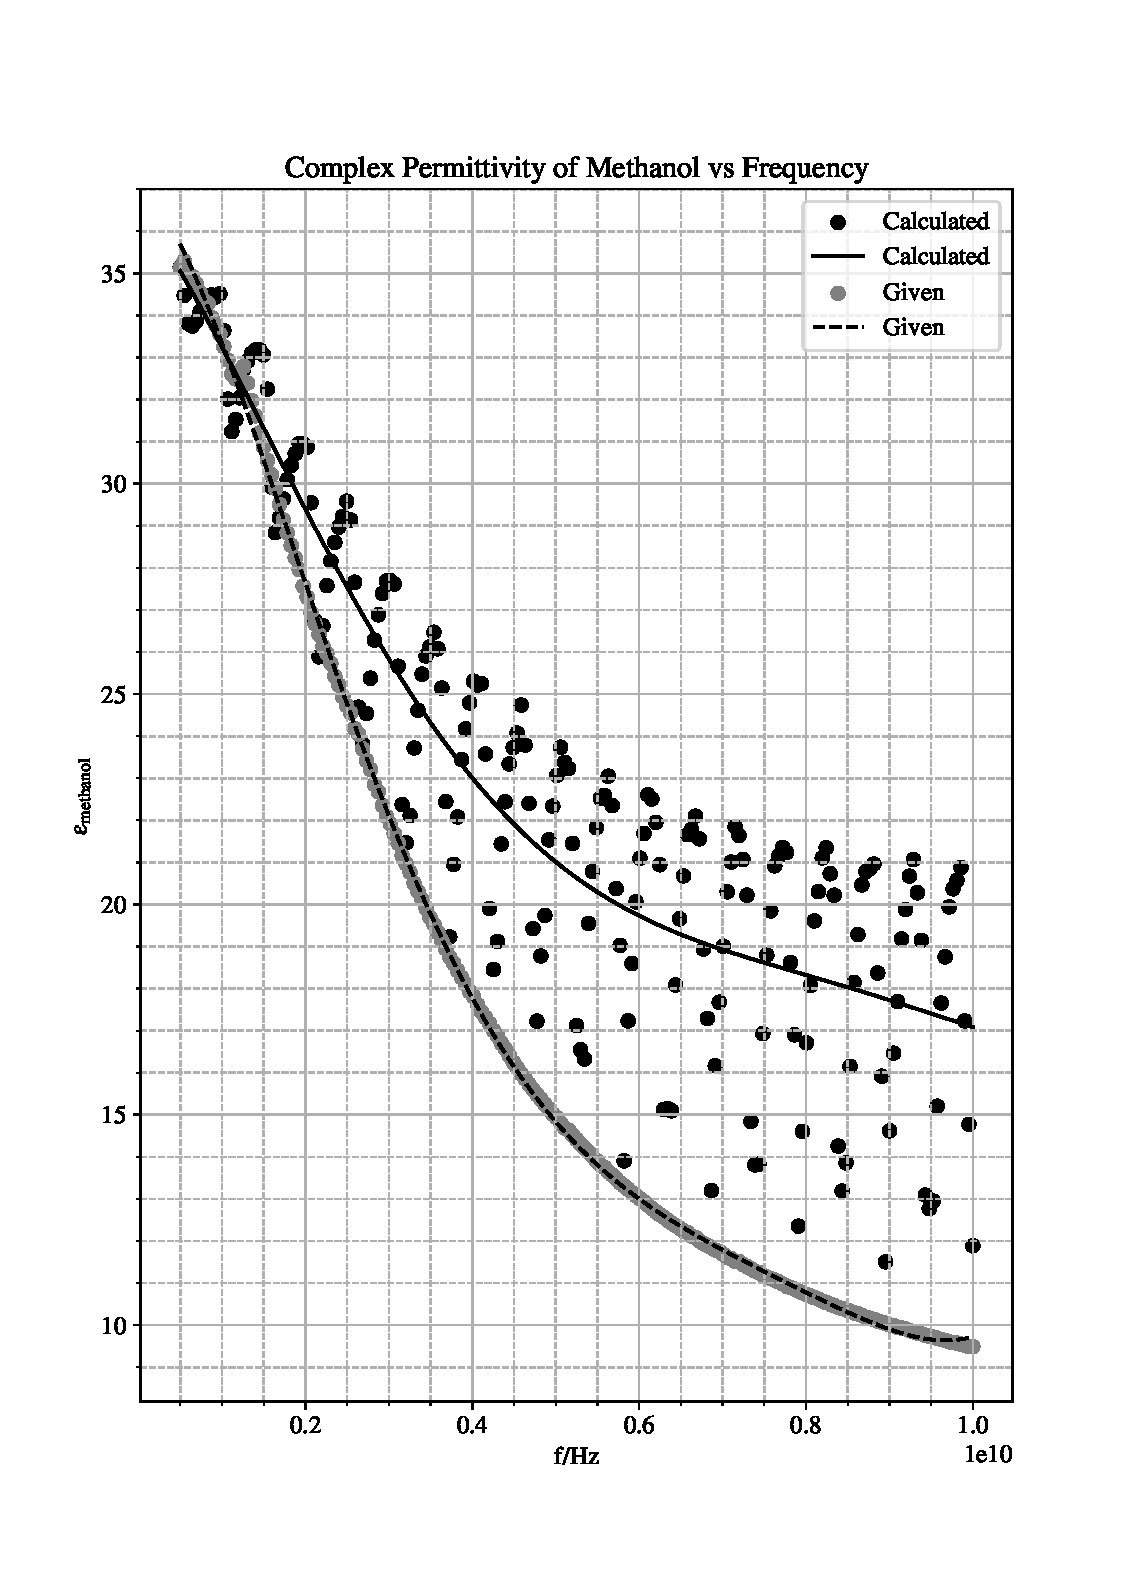
\includegraphics[scale=0.75]{Plot1.pdf}
    \caption{A graph showing stress against strain with a subplot below showing the residuals obtained}
    \end{center}
    \end{figure}


\end{document}
